% =================================================================
% 第3章共享内容：测试环境（以test_detail内容为准）
% =================================================================

% ---------------------------------------------------------------
% 测试环境概述
% ---------------------------------------------------------------

\GjbTestEnvTitleLevelOne{测试环境概述}

本次测试针对xxxxxxxx版本中的xxxxx功能。测试场地在"xxxx601室"。

测试环境包括1台国产ARM架构服务器，2台台式机\ifdefined\GjbEnvFigureLabel如图\ref{\GjbEnvFigureLabel}所示\fi。

ARM架构服务器搭载国产处理器（飞腾），安装国产操作系统（银河麒麟服务器版），安装docker基础环境，安装数据湖xxxx版本。台式机安装Ubuntu 22.04操作系统，安装火狐浏览器。

本次测试环境位于xxxx，测试环境一旦建立并经过确认应保持其状态，任何对测试环境的更改和使用都要进行严格控制,这里做了变更。

\ifdefined\GjbEnvFigureLabel
\begin{figure}[H]
\centering
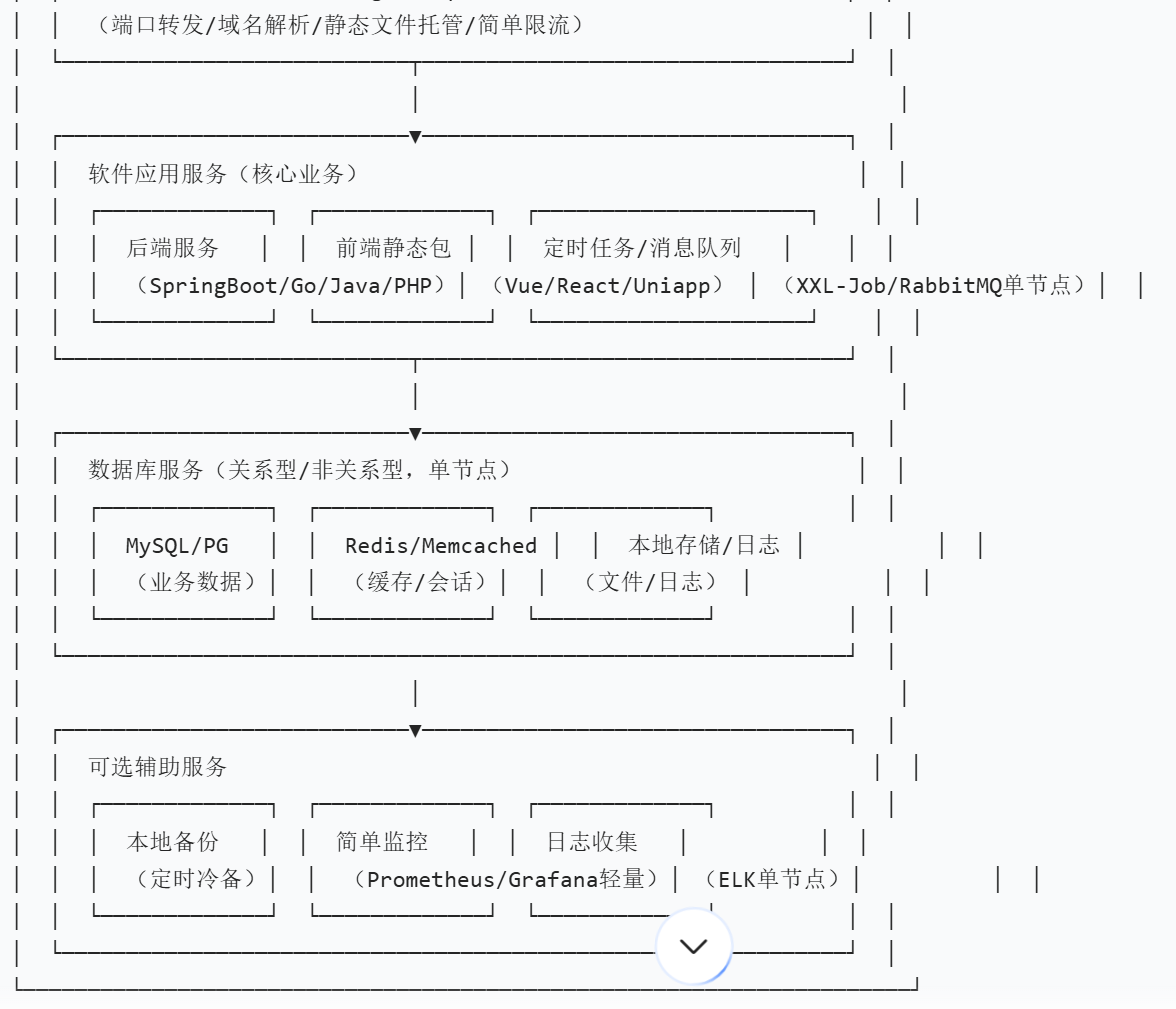
\includegraphics[width=0.9\textwidth]{common/images/environment.png}
\caption{测试环境}
\label{\GjbEnvFigureLabel}
\end{figure}
\vspace{-6pt}
\fi

% ---------------------------------------------------------------
% 软件项
% ---------------------------------------------------------------

\GjbTestEnvTitleLevelOne{软件项}

测试环境中的软件项如表\ref{\GjbEnvSoftwareTableLabel}所示。

{\settablespacing
\begin{\GjbEnvTableType}[theme=gjb,caption={测试环境被测软件},label={\GjbEnvSoftwareTableLabel}]{
  colspec={|p{0.8cm}|p{3.5cm}|p{2.2cm}|p{2.8cm}|p{2.5cm}|p{2.7cm}|},
  rowhead=1,
  hlines={wd=\GjbTableRuleWd,fg=\GjbTableRuleColor},
  cells={halign=c},
}
序号 & 软件名称 & 版本号 & 用途 & 来源 & 存储介质 \\
{\xiaowu 1} & xxxxx & xxxx & 被测软件 & 本单位 & 硬盘 \\
\end{\GjbEnvTableType}}
\vspace{6pt}

{\settablespacing
\begin{\GjbEnvTableType}[theme=gjb,caption={测试环境陪测软件},label={tbl:plan-env-software-support}]{
  colspec={|p{0.8cm}|p{3.5cm}|p{2.2cm}|p{2.8cm}|p{2.5cm}|p{2.7cm}|},
  rowhead=1,
  hlines={wd=\GjbTableRuleWd,fg=\GjbTableRuleColor},
  cells={halign=c},
}
序号 & 软件名称 & 版本号 & 用途 & 来源 & 存储介质 \\
{\xiaowu 1} & 火狐浏览器 & 123.0 & 操作页面 & 开源 & 硬盘 \\
{\xiaowu 2} &  &  &  &  &  \\
{\xiaowu 3} &  &  &  &  &  \\
\end{\GjbEnvTableType}}
\vspace{-6pt}

% ---------------------------------------------------------------
% 硬件和固件项
% ---------------------------------------------------------------

\GjbTestEnvTitleLevelOne{硬件和固件项}

测试环境中的硬件和固件项如表\ref{\GjbEnvHardwareTableLabel}所示。

{\settablespacing
\begin{\GjbEnvTableType}[theme=gjb,caption={测试环境硬件项},label={\GjbEnvHardwareTableLabel}]{
  colspec={|p{0.8cm}|p{1.5cm}|p{1.8cm}|p{2.0cm}|p{0.8cm}|p{2.65cm}|p{1.0cm}|p{2.4cm}|p{1.0cm}|},
  rowhead=1,
  hlines={wd=\GjbTableRuleWd,fg=\GjbTableRuleColor},
  cells={halign=c},
}
序号 & 硬件名称 & 型号 & 编号/序列号 & 数量 & 配置 & 用途 & 软件部署环境 & 来源 \\
{\xiaowu 1} & 服务器 & 长城 & / & 1 & CPU：FT-2000+ *2 内存：256G & 测试机 & 操作系统：Kylin V10，docker & 本单位 \\
{\xiaowu 2} & 台式机 & 联想Think station & / & 2 & CPU：Intel Corei7-12700 内存：32G & 测试机 & 操作系统：Ubuntu 22.04，docker & 本单位 \\
\end{\GjbEnvTableType}}
\vspace{-6pt}
